\section{Practical case study}
\label{sec:gns3practicalcasestudy}

Here will be described the process and results of the experiments carried out to assess aspects of the feasibility, and convenience, of using GNS3 in a real context of teaching and learning a computer networks subject in the University.
Hopefully, some of the gained insights can be extrapolated for other similar teaching facilities of slightly different characteristics.

To provide a real and well-defined set of examples to put in practice, the selected exercises and lab descriptions were taken out of the lab classes handouts for the 2018-2019 edition of ``Architecture and Protocols of Computer Networks,'' known by its Portuguese acronym APRC, an optional, graduate course offered at the Masters in Informatics at the FCT/NOVA.

\subsection{Overview of the considered labs and exercises}
\label{subsec:gns3consideredlabs}

Out of the 5 lab assignments, some of which span across more than one class, planned for a semester, only the first ones, which resort to the lab equipment to put in practice the subjects related to switching and layer-2 and ``legacy'' routing, as opposed to SDN, were considered. % TODO "span across?". Usar esta nota para pôr, se tiver ficado esquecido, referência no trabalho futuro aos exercícios de SDN que podem tirar partido de GNS3 e afins. SDN tem tem de estar nos acrónimos e glossário
Those are the exercises that, in the present, are expected to be done in the lab room, with real interconnected Cisco devices, issuing commands to the IOS command-line interface from the students' laptops.

The so-called ``lab-assignment1'' has a part to introduce the Cisco IOS and some basic commands for it.
Those are the ones to enter and escape the privileged mode, list the device's interfaces, and some other queries.
It also informs of how to load the running configuration of the device into the non-volatile memory, so that it persists after a shutdown, and how to do the opposite to discard unsaved running configurations and load the ones from the nonvolatile memory.

The second handout, ``lab-assignment2,'' is all about switching and layer-2 functionality.
It proposes a topology, expected to map the real interconnecting and physical disposition of devices in the room, of the nine switches, labels them with ``areas'' corresponding to cardinal points.
Students are then guided to answer questions about the expected behavior, e.g. in terms of reachability between hosts, according to parameters, which they should also issue in a coordinated fashion, for STP, VLANs, and trunks.
In figure~\ref{fig:gns3-aprc-lab2-handout-topology}, a section of the document is shown to illustrate the topology, later transfered to GNS3.
The topology has loops which STP is expected to eliminate by disabling certain link(s).
Part of the exercise is to foresee, according to the protocol's specification, which one(s) will be shutdown.

% Figures fig:gns3-aprc-lab2-handout-topology
\begin{figure}
  \centering
  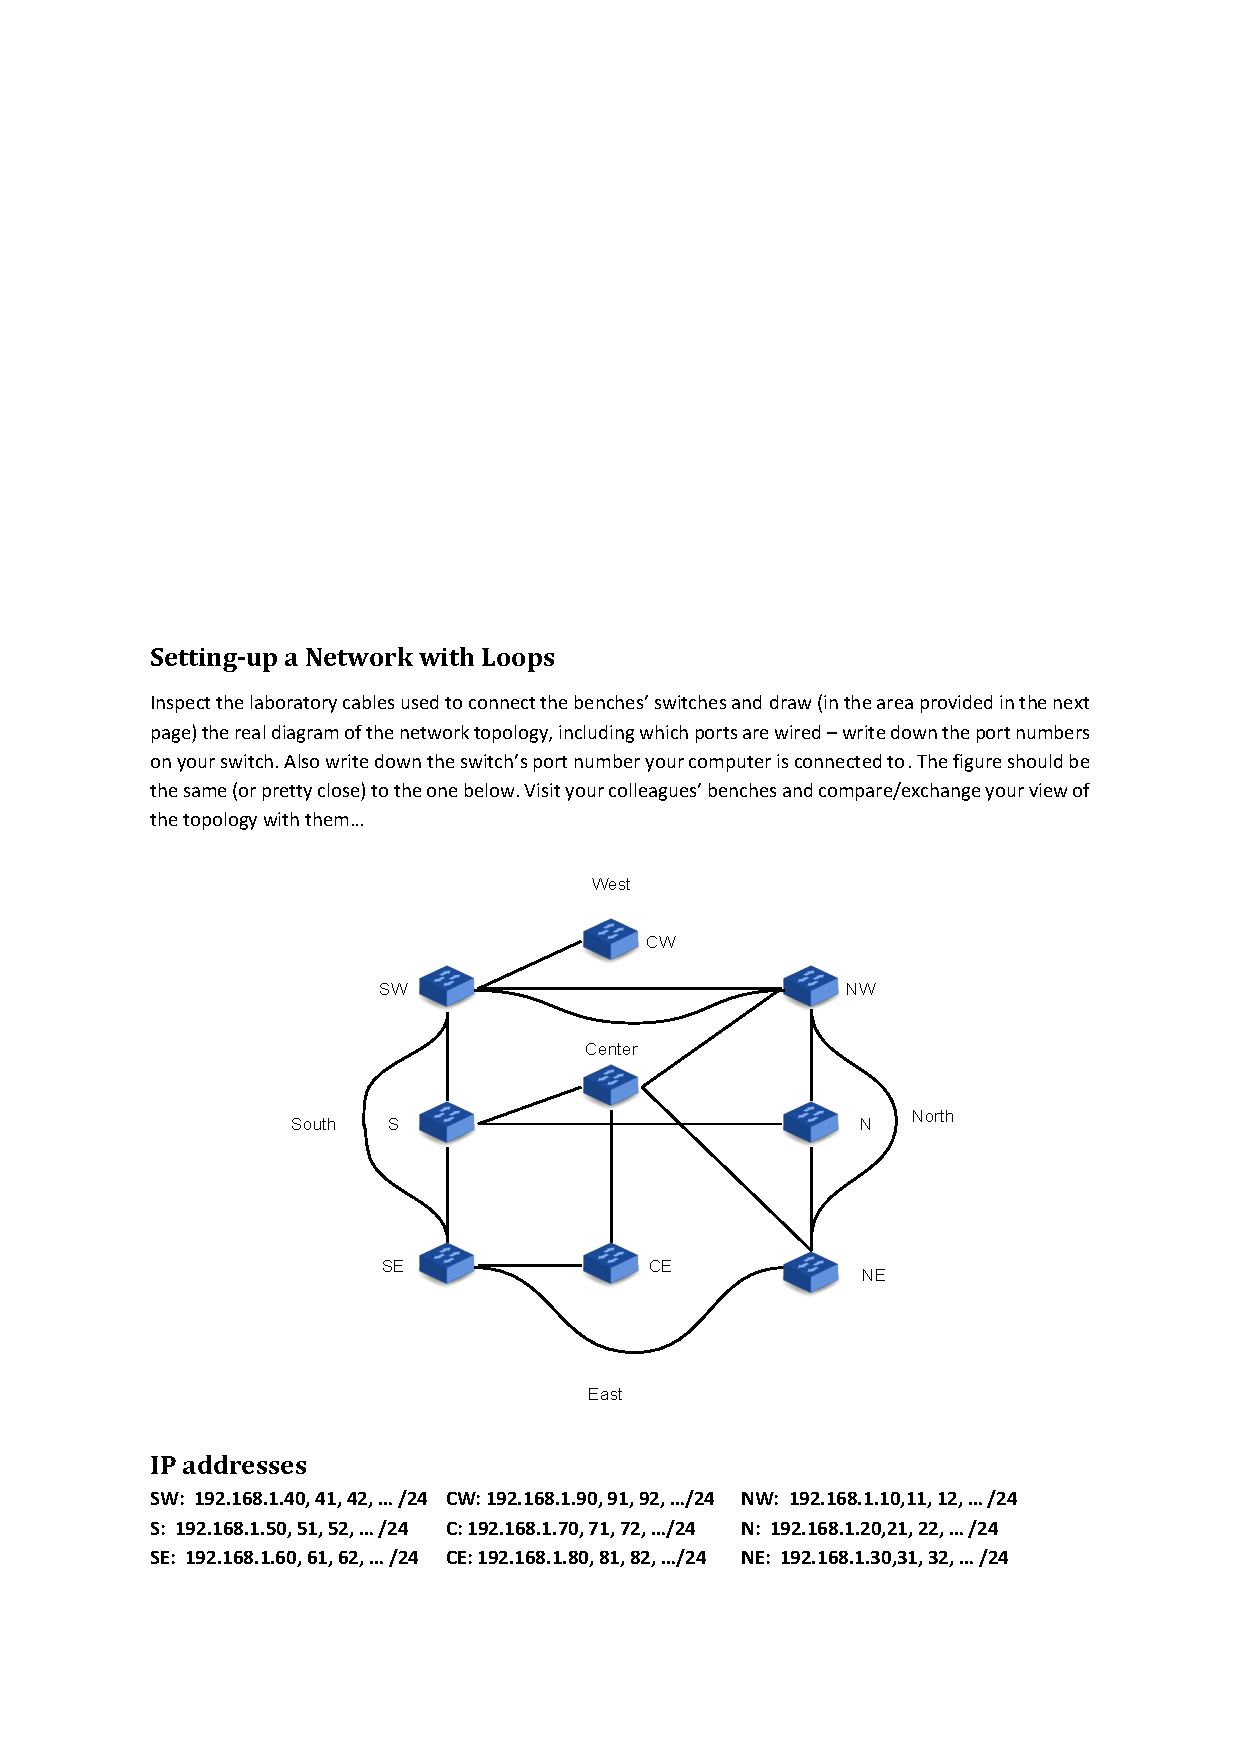
\includegraphics[width=0.8\textwidth, frame]{gns3-aprc-lab2-handout-topology}
  \caption{Section of ``lab-assignment2'' showing the topology}
  \label{fig:gns3-aprc-lab2-handout-topology}
\end{figure}


\subsection{Introduction to Cisco IOS and switching labs}
\label{subsec:gns3introswitching}

As was said before, the first lab assignment introduces host-side commands (mostly Linux) and TCP/IP practical concepts such as IP address and \acrshort{mtu}, and its definition for the host's \acrfullpl{nic}.

% end of section gns3practicalcasestudy
